%%
%% Author: Dario Chinelli
%% begin 2019-12-04
%% last mod 2022-02-21
%%

% Preamble
\documentclass[class=article, crop=false]{standalone}

% Packages
\usepackage[subpreambles=true]{standalone}
%\usepackage{import}
\usepackage{graphicx}
\usepackage{amsmath}

% Document
\begin{document}

In this study, a total of four models are considered. 
Two of them are dependent by the position in space, also called \emph{time-independents}. 
The others two are dependent by the position and time, also called \emph{time-dependents}.
However, there is also a distinction between the D2Q9s and the D2Q9Q9s. 
For the D2Q9s what it is doing is considering the velocity from a cell to another; therefore, just the change in position. 
For the D2Q9Q9s, it is also considering the acceleration; hence, the change in velocity. 
The starting point of each one is the dataset, collected from a real-life situation.

Since each of them are entirely based on real world pedestrian’s path in a crowd, those models considers the imposed limit due to the presence of other pedestrians;
an example of this limit could be the tendency of other pedestrians to not collide with each other and it also considers the boundary condition given by the structural environment. 
The strong point of this model is that it is generated by the real-world observation and not build by hand. 
With the aim of reproducing realistic pedestrians’ movements, synthetic paths are created from the models. 
Every model generates one trajectory that simulate just one pedestrian in a statistical crowd. 
When simulating more paths, it considers pedestrian who walks alone in the crowd. 
This model does not consider the interaction made by the others simulated pedestrians.


\paragraph{Notation}
Lets call the observation field $\Omega_c$, defined as a continuous space where pedestrians are tracked.
Lets assume $\gamma=\gamma( \vec x_c, t)$ a pedestrian's path, where $\vec x_c = (x_c, y_c)$ has a bi-dimensional spacial and time dependancy.

The path $\gamma$ in that space has a start position $A$ and an end position $B$. 
Then, the field $\Omega_c$ is divided into \emph{rectangular} cells, dividing the real space along $x$ with a maximum extension indicated as $Lx$ in a certain number of cells $Dx$; 
the division happens as well for the $y$-direction, with obvious notation: $L_y$ and $D_y$.
After this discretization, from $\Omega_c$ is obtained a \emph{grid space} called $\Omega_g$. 
In this grid space, every path $\gamma$ is converted from continuous $\gamma=\gamma(x_c, y_c, t)$ to discrete coordinate  $\gamma=\gamma(x_g, y_g, t)$ referred to the \emph{grid}. 
To lighten up the notation, while speaking of \emph{grid space}, it is simply used $(x, y)$ in reference to the discrete grid position.


\paragraph{The standard D2Q9 configuration}
Referring to (Figure \ref{fig:D2Q9_k}), the \emph{map} is set for each position $(x_0, y_0)$ in the grid space, and it represents the eight neighbors and the central position where a pedestrian could go. 
Each direction will be associated to a certain transition probability. 
	\import{draw/}{D2Q9_directions_coordinates}
When a trajectory change position, in the grid space (Figure \ref{fig:D2Q9_c}), from $P_0=(x_0, y_0)$ to $P_1=(x_1, y_1)$ is associated a transition. 
The transition is identified by a number $k = 0,1,...,8$ such that is unique. 
It is derived from the series of coordinates for each trajectory and each step in time. 
When the calculation is made for each step, a transition number is also associated for every position in time; this number represents where the position is going to go in the next step.
If this transition is associated to the change in position, it identifies a certain velocity, such as a vector with a certain direction. 
	\import{draw/}{illustrate_eg_path}
From (Figure \ref{fig:Thesis_D2Q9andQ9.001})  to  (Figure \ref{fig:Thesis_D2Q9andQ9.015}), some of the possible changes between cells are shown. 
Those movements may start going $Up$ and evolve in very different ways. 
The First and the Second example start with the same first transition but diverge in the second movement; this leads to two different ending positions. 
Anyway, those transitions have something in common even if they end up in different positions. 
This type of information is contained in the \emph{D2Q9Q9} type of models and not in the \emph{D2Q9} types. 
This lead to different \emph{interpretations} of what is the expectation in that ending position.

Iterating this procedure to the entire pedestrian’s trajectory, it is possible to get something similar to what is illustrated in (Figure \ref{illustrate_eg_path}). 
In that figure, it is possible to distinguish the path in the continuous space and the discrete path in the grid space. 
It also shows the direction of the next movement for each position, using arrows that are consistent with the velocity arrows in each position. 
The numbers are the value of the $k$-index in each position, and they are solid with the maps above. 
This leads the discussion directly to the first model $D2Q9$ in the next paragraph.
	\import{draw/}{eg_grid_transitions}


\paragraph{Model's order of magnitude}
The mathematical framework, generated from each model, is conceptually similar to each other, but their dimensions are pretty different. 
Considering the same field $\Omega$ with same dimensions, it is easy to see that the order of magnitude of the entries’ number rapidly increases, changing the acquisition method.
For example, in the following paragraphs, it is given a similar field space of $200\times100$ cells and a time space of $200$ time-steps to compare all the four model’s tensors by their intrinsic dimensions.


%% --- SECTION SEPARATOR---
\FloatBarrier
\subsection{Model D2Q9} \label{chap:Model_D2Q9}

The simplest model considered here is called \emph{D2Q9-model}. 
This model is time-independent, and it considers the velocity of the pedestrian. 
Given a starting position $(x_0, y_0)$ in the field $\Omega$, it uses the nine closest possible positions a pedestrian could go to from that point. 
Then, through the D2Q9-model, it is possible to know, for each position $(x_0, y_0)$, the probability to go up, down, left, right or a combination of those movements.



\paragraph{Transitions} 

From the initial position $P_0=(x_0, y_0)$ to the next closest cell in the grid, $P_k$ is defined by the index $k$; in this way, the index k gives the direction of the transition. 
To explicit all the transitions from $P_0$ to $P_k$, those transformations are defined in (Equation \ref{eq:transitions_D2Q9}) and represented as diagram (Figure \ref{fig:D2Q9_k_arrow}):
\begin{equation}
\begin{split}
P_0 &\to P_0 : \quad (x_0, y_0) \to (x_0, y_0) \\
P_0 &\to P_1 : \quad (x_0, y_0) \to (x_0+1, y_0) \\
P_0 &\to P_2 : \quad (x_0, y_0) \to (x_0, y_0+1) \\
P_0 &\to P_3 : \quad (x_0, y_0) \to (x_0-1, y_0) \\
P_0 &\to P_4 : \quad (x_0, y_0) \to (x_0, y_0-1) \\
P_0 &\to P_5 : \quad (x_0, y_0) \to (x_0+1, y_0+1) \\
P_0 &\to P_6 : \quad (x_0, y_0) \to (x_0-1, y_0+1) \\
P_0 &\to P_7 : \quad (x_0, y_0) \to (x_0-1, y_0-1) \\
P_0 &\to P_8 : \quad (x_0, y_0) \to (x_0+1, y_0-1) \\
\end{split}
\label{eq:transitions_D2Q9}
\end{equation}

	\import{draw/}{D2Q9_directions_arrows}
Considering the (Figure \ref{fig:D2Q9_k_arrow}), all the transitions are associated to a specific $k$. 
This is a particularly simple Markov Chain in which there are a total of \emph{nine} states. 
Between these states, the transitions always and only start from the $P_0$ state to go to the others $P_k$ states or itself. 
The same concept is graphically represented with the diagram in (Figure \ref{diagram:diagram_MC_D2Q9}). 
To every transition, it is associated a certain probability of that transition to happen. 
Formally, this probability is given by the initial and the final states: $p_{if}$. 
Since the starting state always stays the same, it is possible to omit it. 

Therefore, the probability of the transition from $P_0$ to $P_k$ is expressed by $p_k(x, y)$, where the index $k$ points to the ending state. 
It means that for each position in $\Omega$, it is possible to say how likely is to “step forward” or “turn right” and so on. 
Then, once it is in the new position, it is again possible to say the most probable direction the pedestrian will choose. 
The same prediction is applicable to the whole space, mapped by the real data.
	\import{draw/}{D2Q9_MarkovDiagram}


\paragraph{Tensor's dimension}
With this structure it is possible to create a tensor $A$ with three indices.
Taking into account the simplest model, as above, the relative \emph{tensor} is $A_{x y k}$.
Where every entries is the probability $p$ to move along the $k$ direction from the location $(x, y)$.
The total number of elements in $A$ is the product between: 
\begin{equation*}
\begin{split}
N(A_{xyk}) &= \mbox{(dim-x-grid)} \times \mbox{(dim-y-grid)} \times \mbox{(dim-k-array)} \\
& = \mbox{(dim-x-grid)} \times \mbox{(dim-y-grid)} \times 9
\end{split}
\end{equation*}
e.g. in the following paragraphs is used a grid space of $200\times100$ cells, so the number of entries would became 
\begin{equation*}
\begin{split}
N(A_{xyk})=200\times100\times9 = 180000 \; .
\end{split}
\end{equation*}
Since the aim of every models is to simulate a pedestrian in the crowd, this tensor is the key to get to the result.
In general it's not easy to represent the tensor $A$ in all following models, but it's possible for this first one as plotted in (Figure \ref{fig:TensorA_D2Q9}).
It shows a $3\times3$ matrix of figures.
Each one is referred to a certain value of the $k$-index.
Each figure's position is in reference to the usual $D2Q9$ map, similarly as in (Figure \ref{fig:D2Q9_k}).

\begin{figure}[h!]
\centering
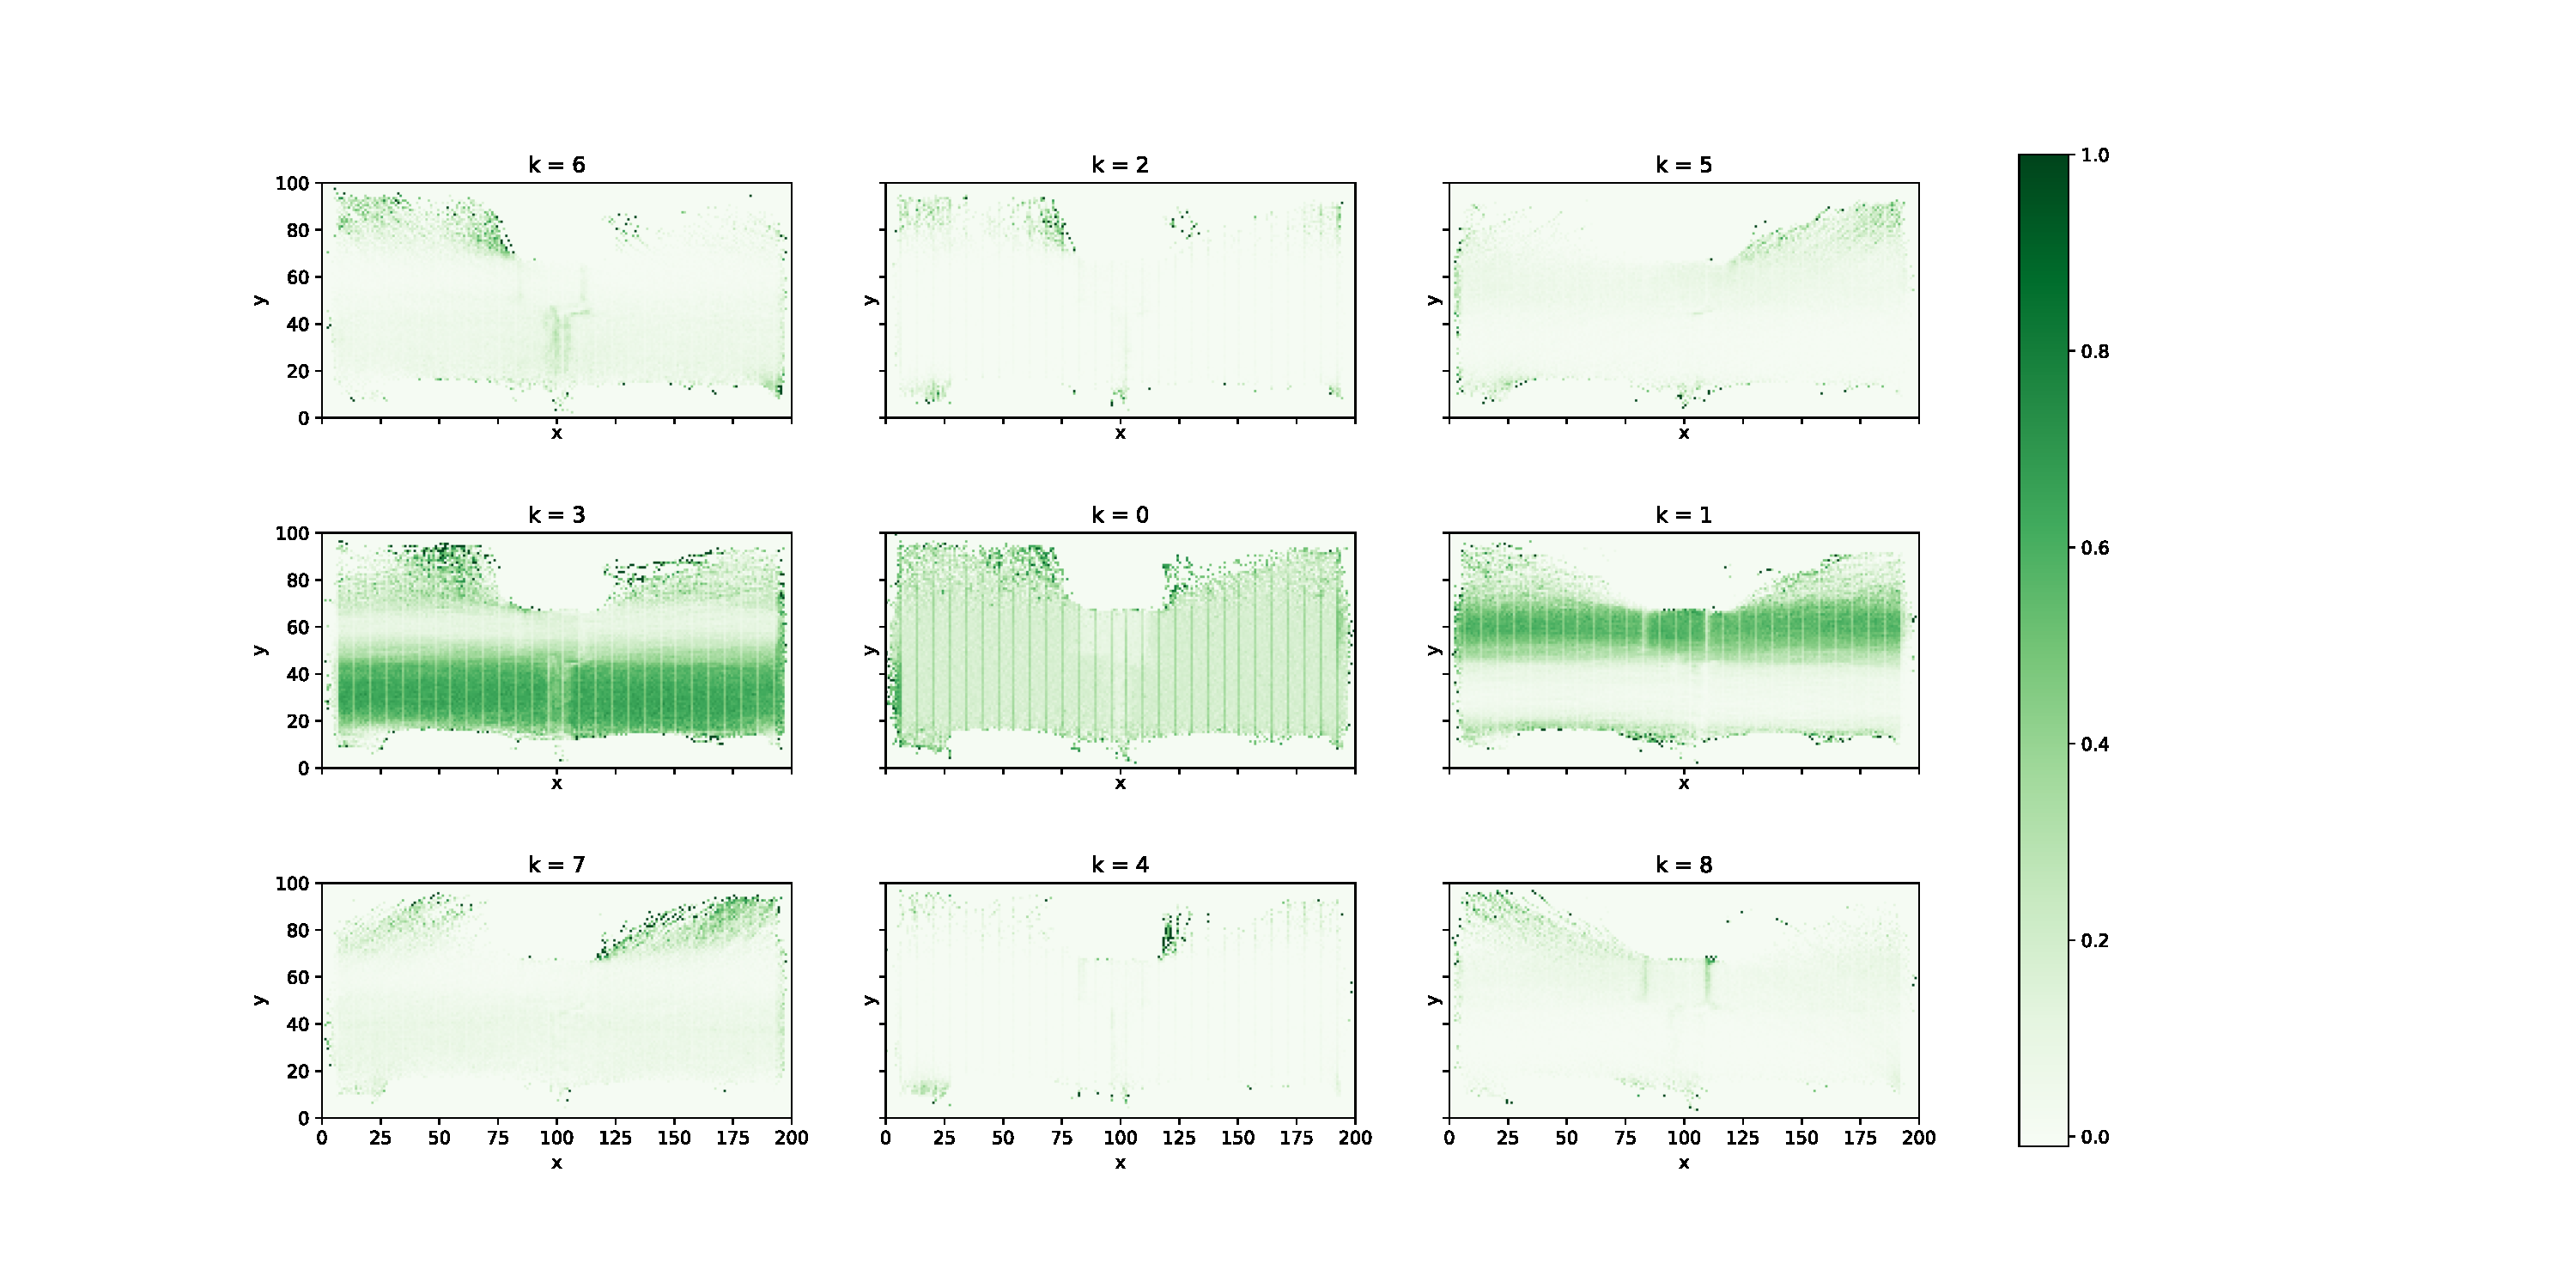
\includegraphics[scale=0.35]{fig/figure_trainf10_all_trajectories_Dx200_Dy100_TensorA_D2Q9}
\captionsetup{width=.6\linewidth}
\caption{Each figure represents the probability in every position to move along a certain direction, defined by the $k$-index.}
\label{fig:TensorA_D2Q9}
\end{figure}


%% --- SECTION SEPARATOR---
\FloatBarrier
\subsection{Model D2Q9Q9}
The conceptual step forward of the study is to consider the next position, but also the previous one.
Similarly to the previous model, this is a \emph{time-independent} model.
Hence given a trajectory $\gamma$ in the grid space of a pedestrian that make a transition for each time step.
For each point $P_0$ of $\gamma$ it is possible to determinate where it was before at $P_{-1}$ and where is going to be after at $P_{+1}$.
The index that represents the \emph{next} position is $k$, meanwhile the index that represents the \emph{previous} position is $h$.
For instance it is given the table of the coordinates and the two indexes related to the (Figure \ref{diagram:diagram_MC_D2Q9}) in the (Table \ref{table:diagram_MC_D2Q9}).
\begin{table}[h!]
\centering
\begin{tabular}{|c|c|c|c|c|}
\hline
Time step & $x_g$ & $y_g$ & $k$-index & $h$-index  \\ \hline
1         & 5 & 1 & 3 & 0 \\ \hline
2         & 4 & 1 & 2 & 1 \\ \hline
3         & 4 & 2 & 3 & 4 \\ \hline
4         & 3 & 2 & 2 & 1 \\ \hline
5         & 3 & 3 & 5 & 4 \\ \hline
6         & 4 & 4 & 2 & 7 \\ \hline
7         & 4 & 5 & 2 & 4 \\ \hline
8         & 4 & 6 & 2 & 4 \\ \hline
9         & 4 & 7 & 2 & 4 \\ \hline
10        & 4 & 8 & 6 & 4 \\ \hline
11        & 3 & 9 & 0 & 8 \\ \hline
\end{tabular}
\captionsetup{width=.6\linewidth}
\caption{This is tabulated the trajectory of the same illustrative pedestrian as above in (Figure \ref{diagram:diagram_MC_D2Q9}).
Here is expressed the position time to time, the index of the following move and the index of the previous move.}
\label{table:diagram_MC_D2Q9}
\end{table}

\paragraph{Tensor's dimension}
The \emph{tensor} associated to this model is characterized by a total of four indexes as $A_{x y k h}$.
Every element of this tensor is now representing a certain probability to move away from a state to another, but considering also the previous position.
The total number of elements in $A$ is the product between:
\begin{equation*}
\begin{split}
N(A_{xykh}) &= \mbox{(dim-x-grid)} \times \mbox{(dim-y-grid)} \times \mbox{(dim-k-array)} \times \mbox{(dim-h-array)} \\
& = \mbox{(dim-x-grid)} \times \mbox{(dim-y-grid)} \times 81
\end{split}
\end{equation*}
e.g. in the following paragraphs is used a grid space of $200\times100$ cells, so the number of entries would became 
\begin{equation*}
\begin{split}
N(A_{xykh})=200\times100\times 81 = 1620000 \; .
\end{split}
\end{equation*}
Taking into account the example in the (Table \ref{table:diagram_MC_D2Q9}), and considering this the only one possible trajectory.
It is easy to see that the probability at $A_{x y k h} = A_{3, 3, 5, 4} = 1$ is maximum in the position $(3, 3)$.
The probability for every other $k, h$ in the same position is zero, $A_{3, 3, k, h} = 0 \quad for \, k \neq 5, \, h \neq 4$.
Instead, if two trajectories pass by the same position in the grid but with different directions, this probability is distributed along two directions.
This is the scenario represented in (Figure \ref{fig:two_trj_same_cell}), where there are two trajectories.
Those pass by the same cell at different times, but leave in the model $D2Q9Q9$ a strong influence.
In this case $A_{2, 2, 5, 7} = 1$ and $A_{2, 2, 6, 8} = 1$.
For the previous model $D2Q9$ in the same position it would be, with $A_{x y k}$, $A_{2, 2, 5} = 0.5$ and $A_{2, 2, 6} = 0.5$.
In (Table \ref{table:two_trj_same_cell}) are explicitly expressed the positions and the values of $k$ and $h$ for the two illustrative paths.
\begin{figure}[h]
\centering
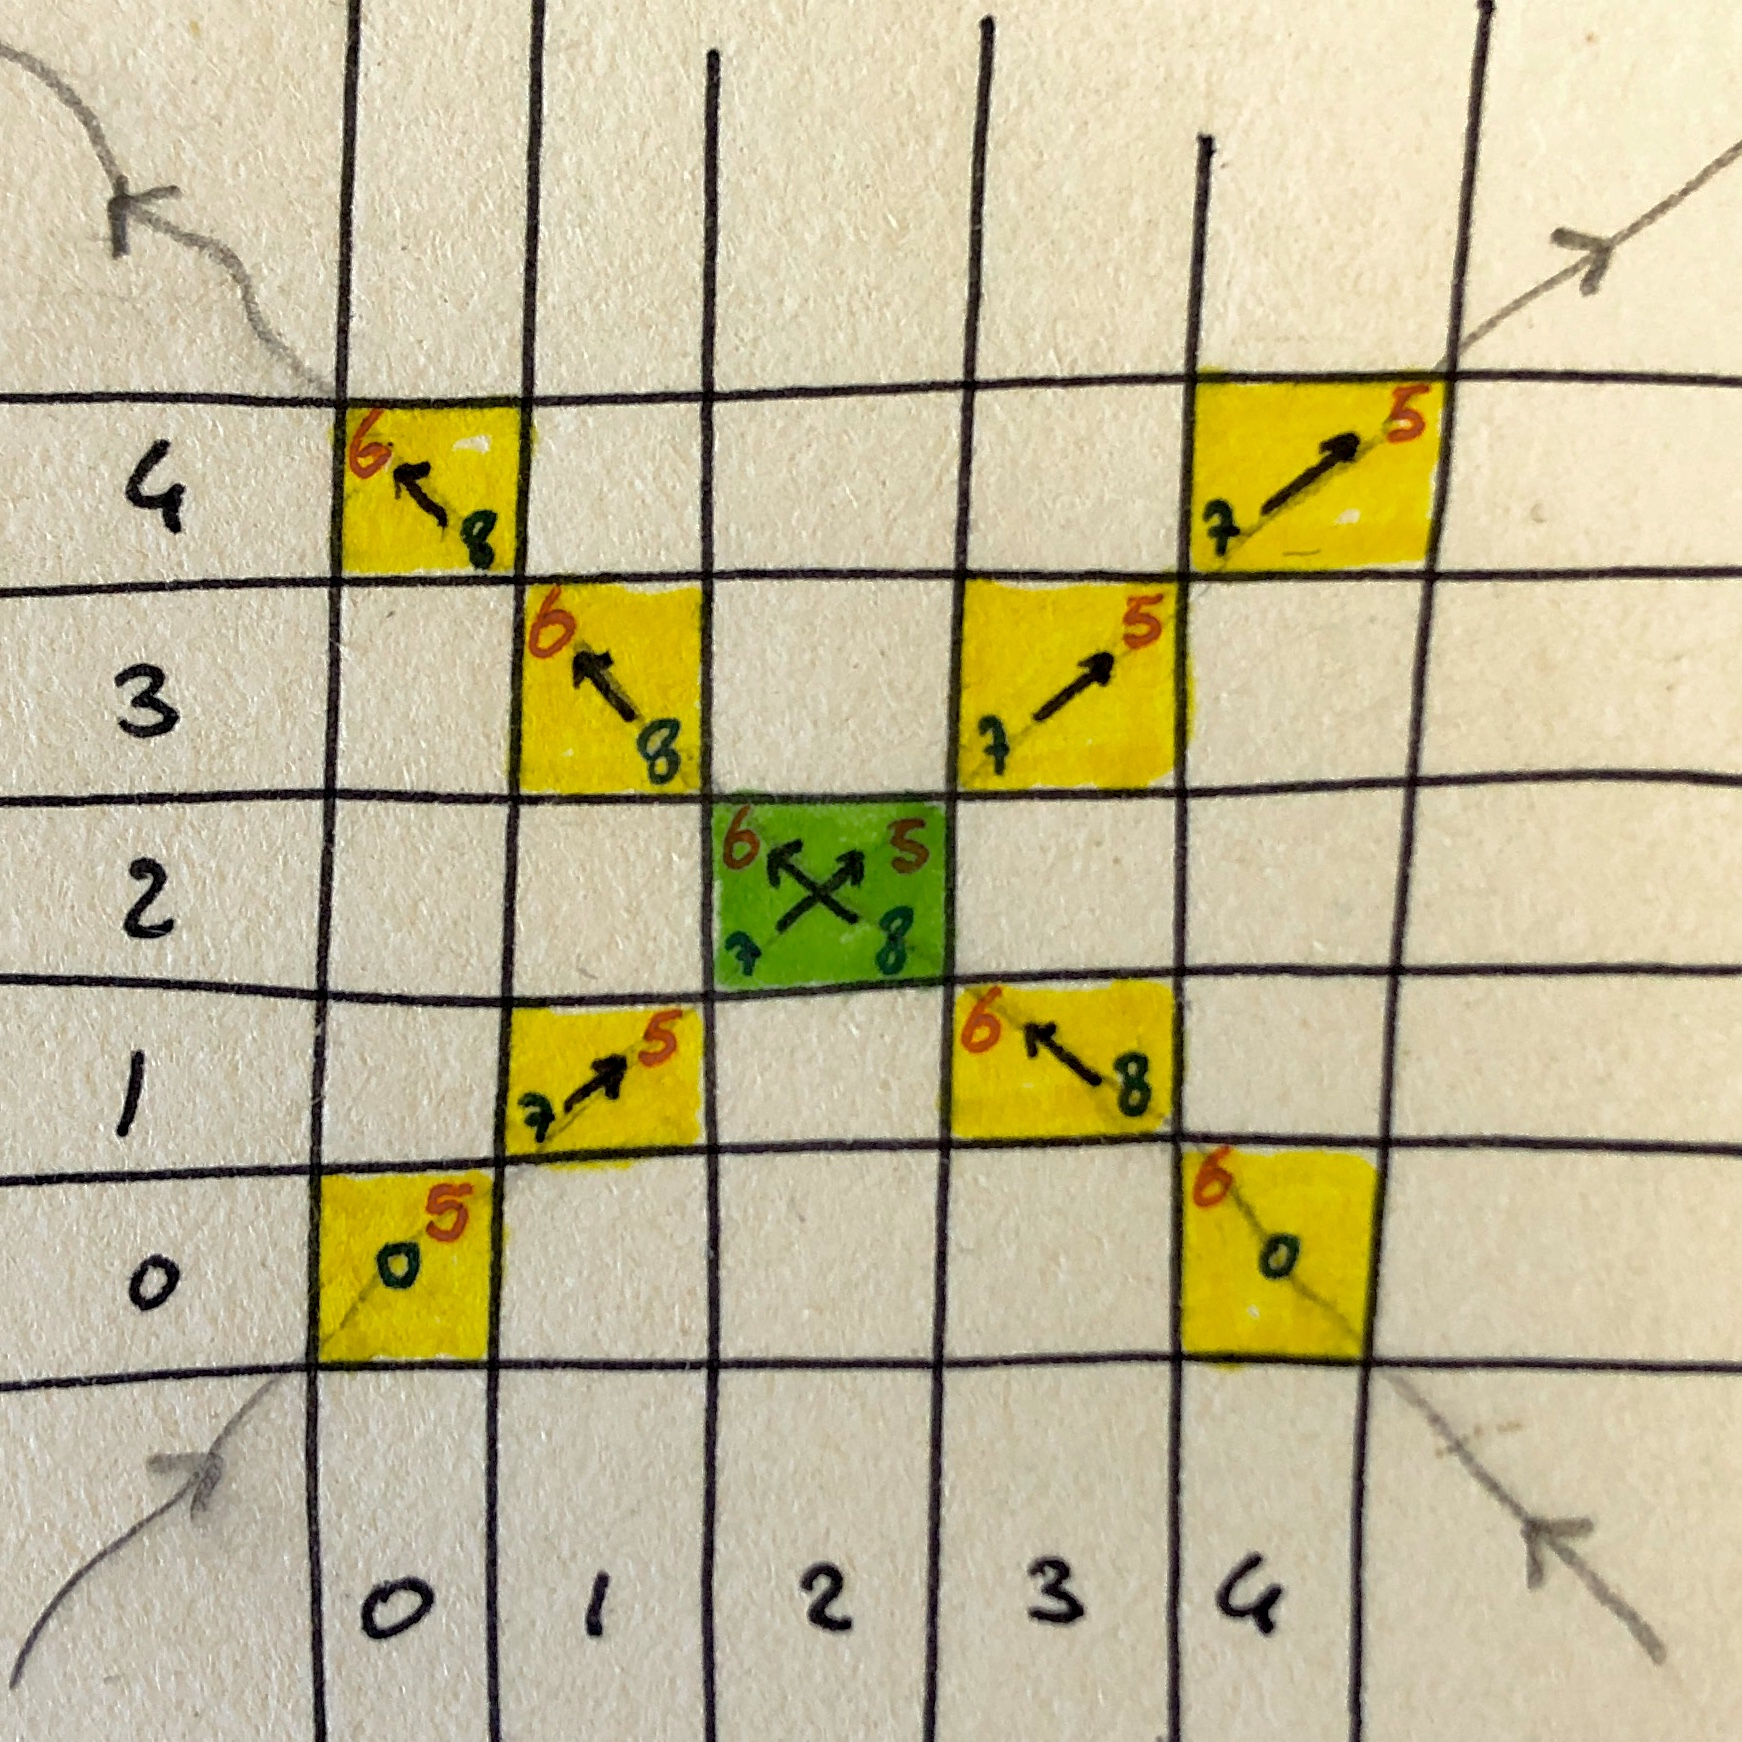
\includegraphics[scale=0.1]{draw/eg_distribution_two_trajectories_1}
\captionsetup{width=.7\linewidth}
\caption{Two paths passing by the same cell, in green, with different directions.
The numbers in red are defining the values of the $k$-index for every step.
The numbers in blue are the values of the $h$-index for every step.}
\label{fig:two_trj_same_cell}
\end{figure}
\begin{figure}[h]
\centering
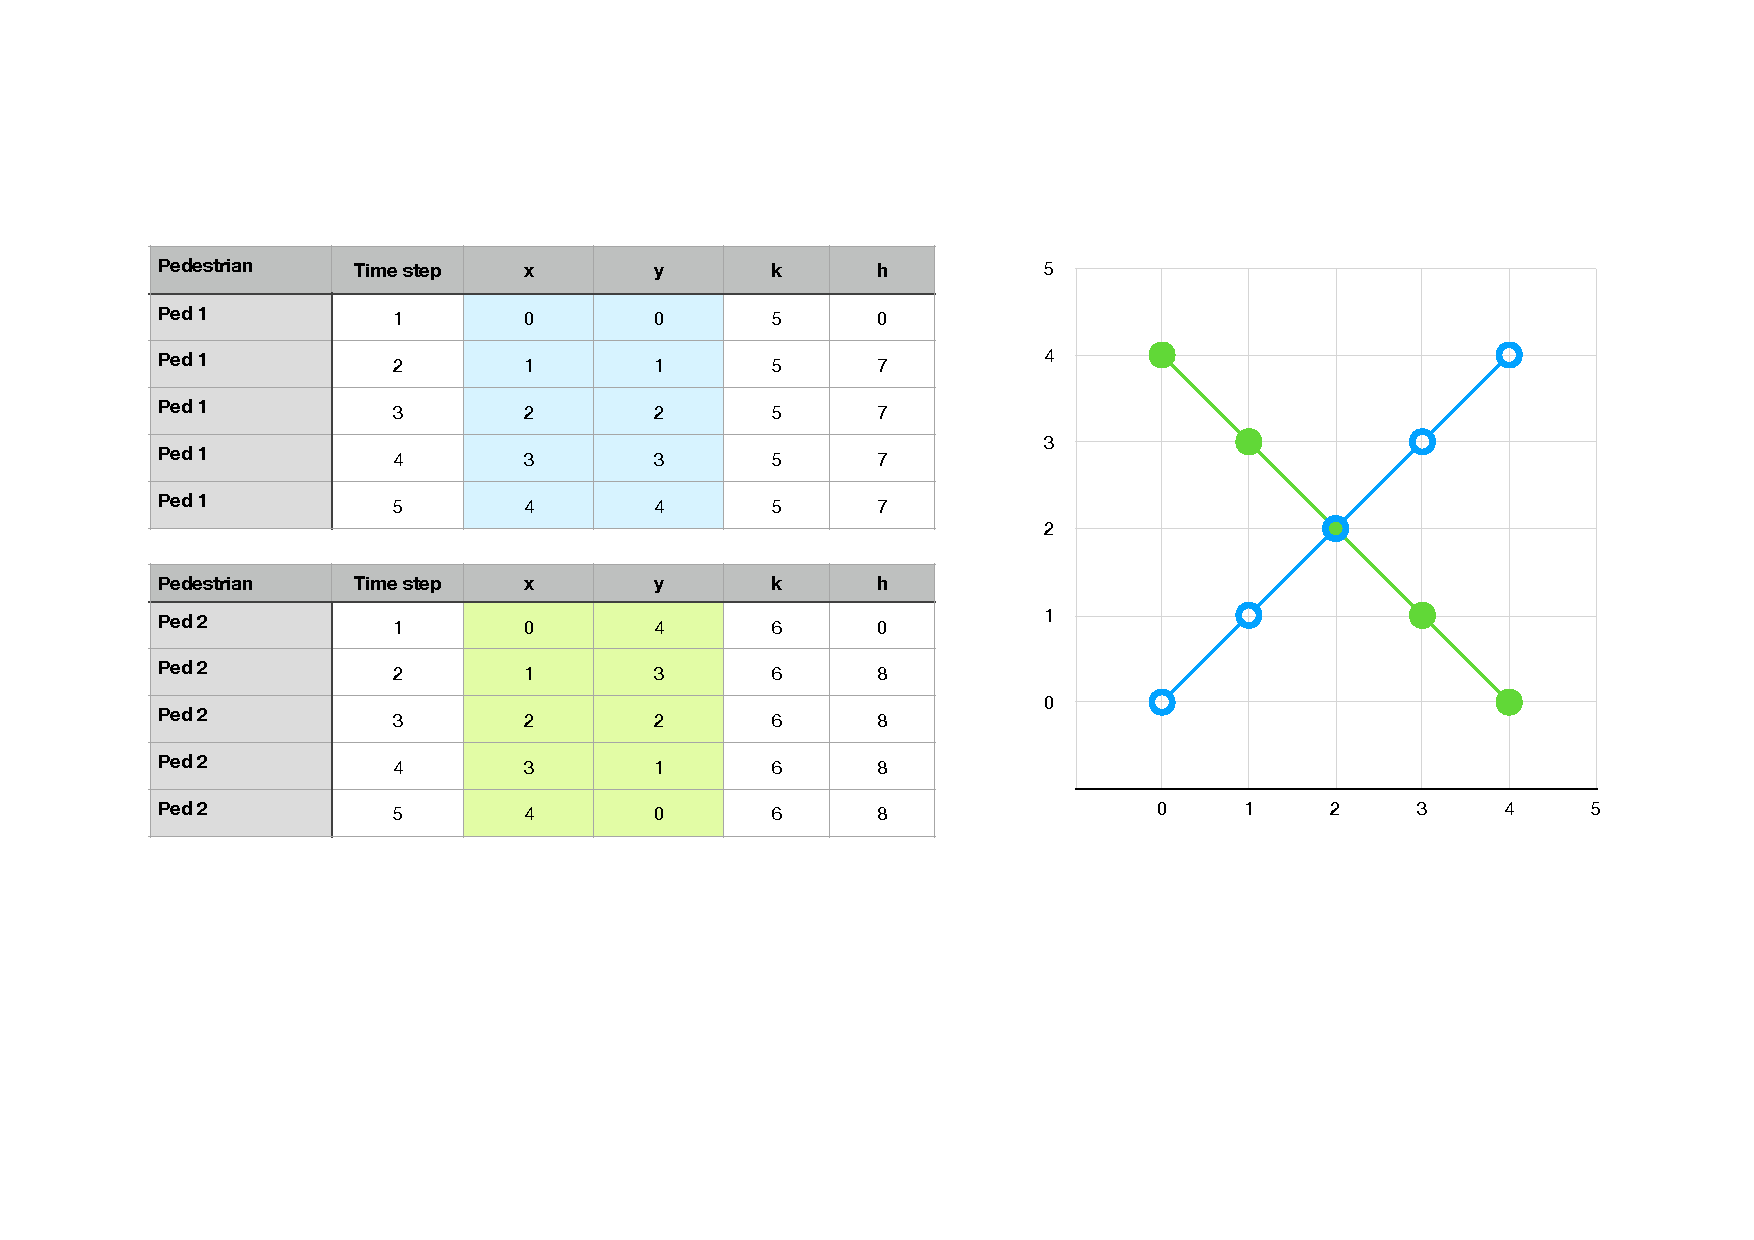
\includegraphics[scale=0.5]{draw/eg_distribution_two_trajectories_2}
\captionsetup{width=.7\linewidth}
\caption{Two paths passing by the same cell, with different directions.}
\label{table:two_trj_same_cell}
\end{figure}

\paragraph{Cross trajectories}
A common situation when looking at the trajectories is to find intersections with two different directions.
Lets take into account the previous example, where two pedestrians cross the field very differently.
One from the left-down to the right-up corners and the other from the right-down to the left-up corners.
The intersection that is formed from this two paths is the highlighted green cell in (Figure \ref{fig:two_trj_same_cell}).
As mentioned before, the simpler model $D2Q9$ has more problems with this situation than the $D2Q9Q9$.
The reason is that for the $D2Q9$ it is taken into account the velocity on a particular cell so it is considering instantaneous direction. 
When simulating pedestrian arrive at that intersection, is inevitable to get a probability to \emph{change} directions and go back.
This situation is one of the deeper reason to change model to $D2Q9Q9$ to take into account also the previous position.
In fact, in this situation a simulated pedestrian would not change direction for the second model, because it has probability zero to make it.

%% --- SECTION SEPARATOR---
\FloatBarrier
\subsection{Model TD2Q9}
This module takes into account all the tools offered by the \emph{D2Q9 model}.
But time is now relevant and so this is a \emph{time-dependent} model.

\paragraph{Time}
It is important to describe properly what is \emph{time} in this study.
Lets start from what is not: time is not the universal time, like UTC.
Time here is discrete and it's defined also as \emph{time step}.
It is divided in seconds, using the \emph{unix time} or \emph{UNIX Epoch time}.
Every step in time define a new state along the time axes, it is possible to imagine it as a new dimension.
For each pedestrian path, time start at the entrance in the field and ends at the exit of it.
So time is relative to each trajectories and not global.

The definition of a \emph{state} is not just by the position in space but is given by $x, y, t$.
In this model, pedestrians moves along three axes: two dimensions in space and one in time.

\paragraph{Tensor's dimension}
The \emph{tensor} representing the probability to move is defined by $A_{t x y k}$.
With this structure it is possible to associate the velocity to the time step.
The total number of elements in $A$ is the product between:
\begin{equation*}
\begin{split}
N(A_{t xyk}) &= \mbox{(dim-time-grid)} \times \mbox{(dim-x-grid)} \times \mbox{(dim-y-grid)} \times \mbox{(dim-k-array)} \\
& = \mbox{(dim-time-grid)} \times \mbox{(dim-x-grid)} \times \mbox{(dim-y-grid)} \times 9
\end{split}
\end{equation*}
e.g. in the following paragraphs is used a grid space of $200\times100$ cells and the mean dimension in time for significants trajectories is dim-time $ = 200$, so the number of entries would became 
\begin{equation*}
\begin{split}
N(A_{t xyk})=200 \times 200\times100\times 9 = 36000000 \; .
\end{split}
\end{equation*}
This gives the possibility to differentiate when a trajectory is going to exit or is just entered, when giving the probability to move.
Lets make an example and consider a position close to the map border $P_b = (x_b, y_b)$, something like in (Figure \ref{fig:boundary_position}).
If it's not known the time of this position $P_b$ the probabilities to go to the center of the map or out of it are non zero.
So it's not possible, given $P_b$, to really distinguish if the pedestrian is going out or not.
But if the time is taken into account it's necessary to distinguish if the pedestrian is at the beginning of it's path or at the end.
Lets start again from the position $P_b$.
If it's at the beginning in time steps, the more probable move will be to the center.
If some time is passed inside the map, it will have higher probability to go out from the map.

\begin{figure}[h]
\centering
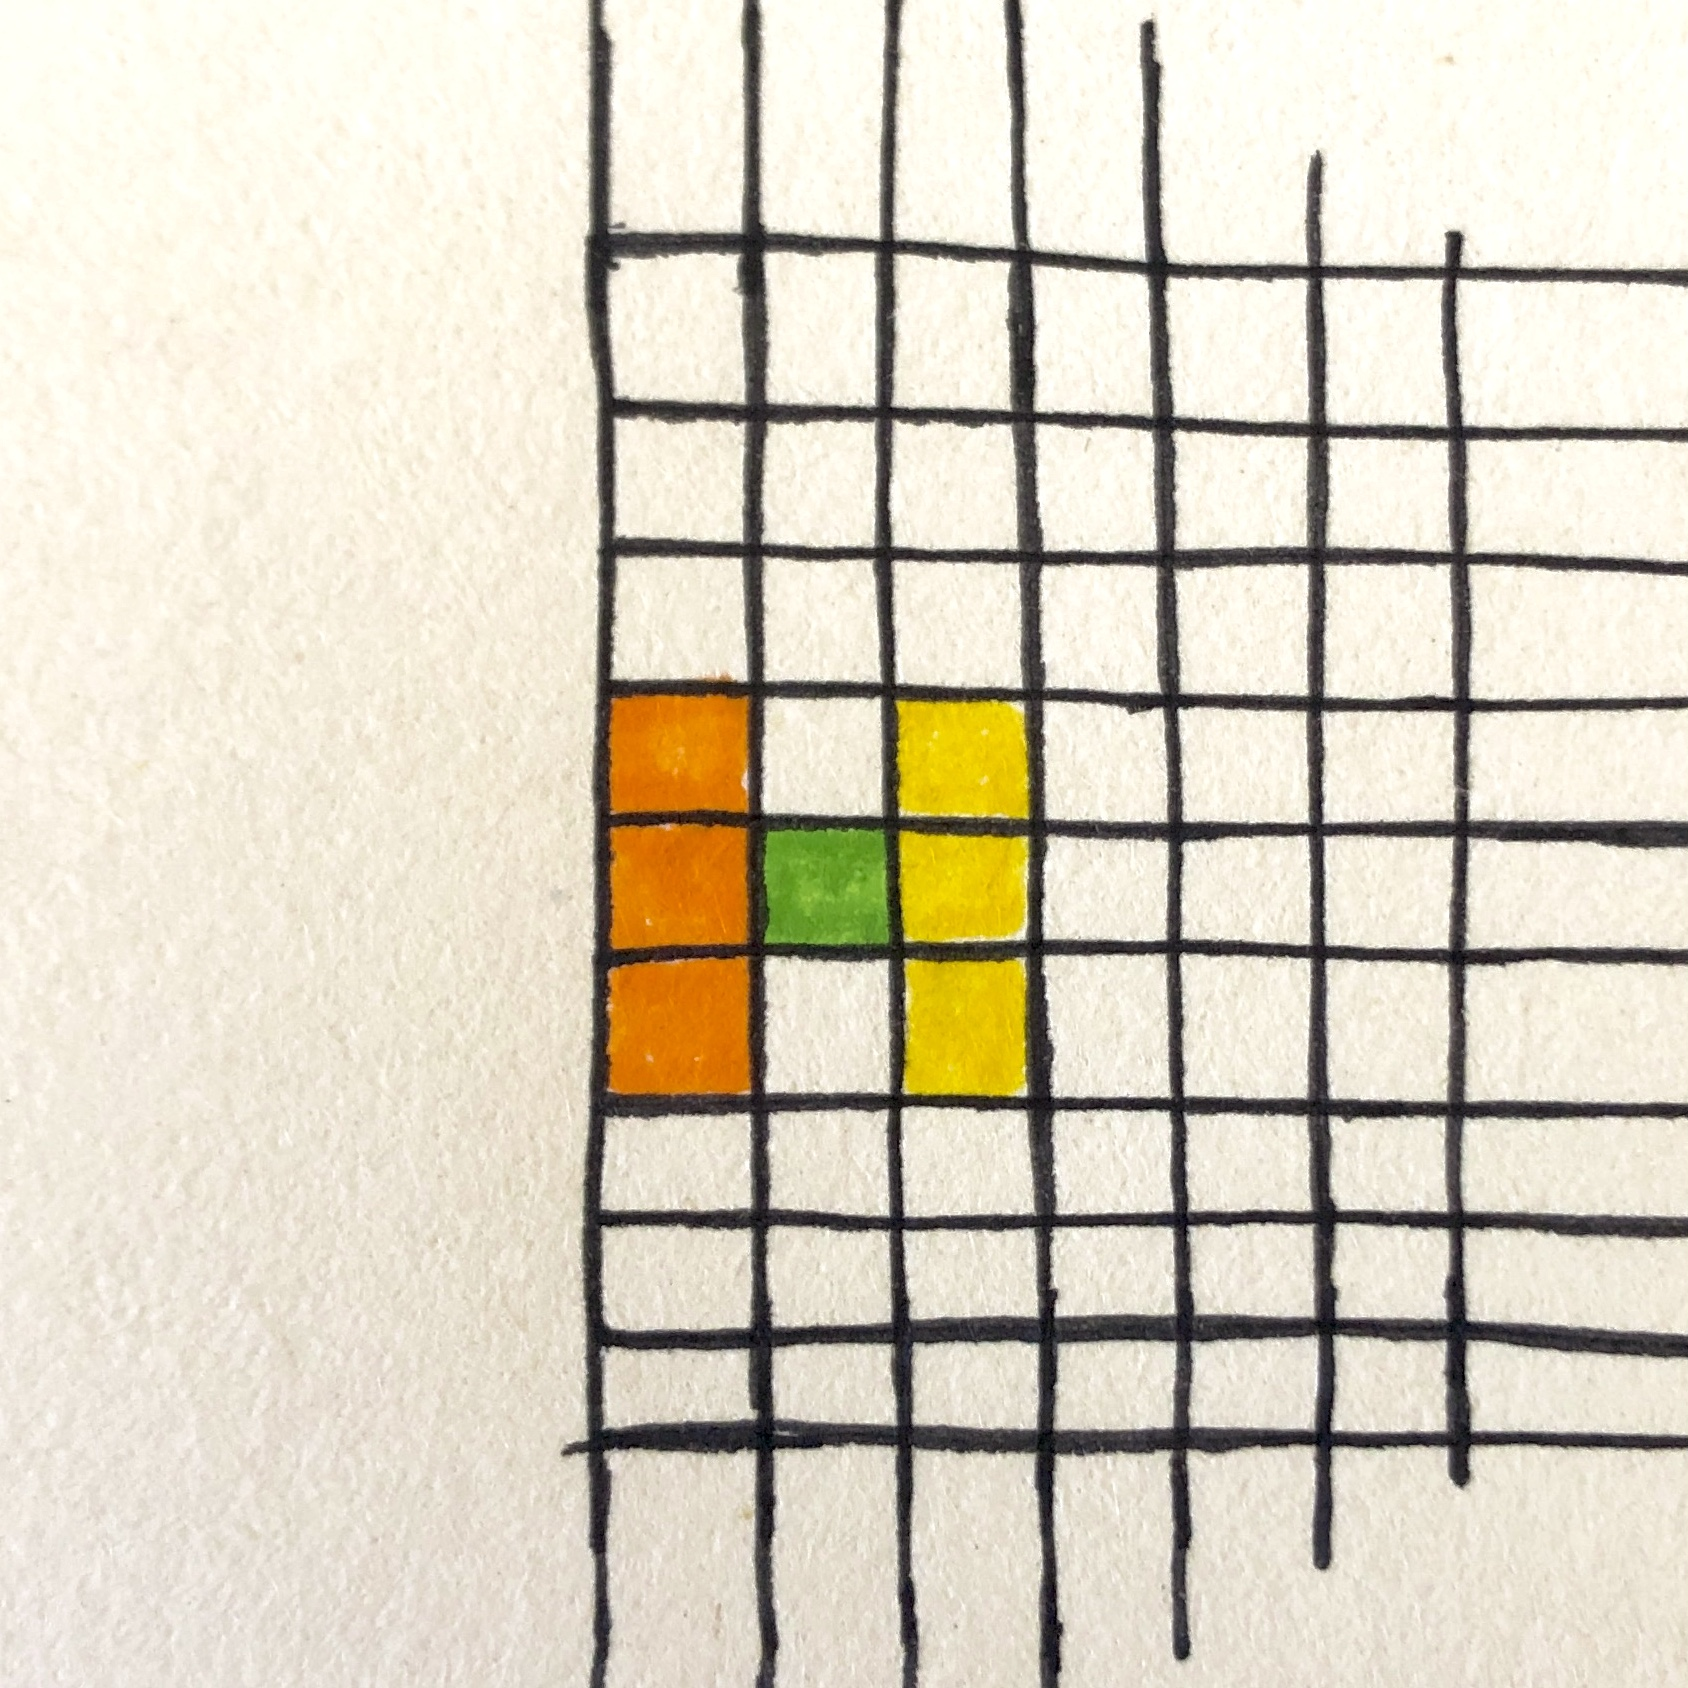
\includegraphics[scale=0.1]{draw/Boundary_position_in_out}
\captionsetup{width=.6\linewidth}
\caption{The boundary position $P_b$ considered is the green cell.
When time is \emph{small}, the trajectory is at the beginning, yellow positions are more likely than orange positions.
When time is \emph{big}, the trajectory is at the ending, yellow positions are less likely than orange positions.}
\label{fig:boundary_position}
\end{figure}


%% --- SECTION SEPARATOR---
\FloatBarrier
\subsection{Model TD2Q9Q9}
This model is the extension of the previous \emph{TD2Q9} and the \emph{D2Q9Q9} method, where time and acceleration are taken into account.

\paragraph{Tensor's dimension}
With this method it is associated a tensor $A_{t x y k h}$, with five dimensions.
With evident notation, in reference to the previous paragraphs, it's dependent on the time $t$, the position $(x, y)$, the future position $k$ and the previous position $h$.
With the $TD2Q9Q9$-model is taken into account the information on acceleration in a position combined to the time of corresponding to that position.
The total number of elements in $A$ is the product between:
\begin{equation*}
\begin{split}
N(A_{t xykh}) &= \mbox{(dim-time-grid)} \times \mbox{(dim-x-grid)} \times \mbox{(dim-y-grid)} \times \mbox{(dim-k-array)} \times \mbox{(dim-h-array)} \\
& = \mbox{(dim-time-grid)} \times \mbox{(dim-x-grid)} \times \mbox{(dim-y-grid)} \times 81
\end{split}
\end{equation*}
e.g. in the following paragraphs is used a grid space of $200\times100$ cells and the mean dimension in time for significants trajectories is dim-time $ = 200$, so the number of entries would became 
\begin{equation*}
\begin{split}
N(A_{t xyk})=200 \times 200\times100\times 81 = 324000000 \; .
\end{split}
\end{equation*}

\paragraph{Time}
As before, time is the proper time of each pedestrian.
It define the time of a certain step along the whole trajectory.

This very last model studied in this work is the most complex but may lead to a more appropriate simulation.
It's also the most computationally expensive because of the great number of items and because it needs a big number of trajectories to \emph{fill} it all.














\end{document}
